The performance of the proposed method has been compared against three other Bengali text summarization methods to evaluate the correctness of generated summaries by using human written summaries as reference. The three methods, which have been used as a benchmark, are BenSumm~\cite{chowdhury-etal-2021-tfidf-clustering}, LexRank~\cite{Erkan-lexRank-2004} and SASbSC~\cite{roychowdhury-etal-2022-spectral-base}. All of these methods have been evaluated using four Bengali extractive text summarization datasets to test the robustness of the method's performance in various types of input. For evaluation of the methods, the Recall-Oriented Understudy for Gisting Evaluation (ROUGE)~\cite{lin-2004-rouge} metric has been used. Details about the models, datasets and evaluation metrics are provided in the following sections.

\subsection{Text Summarization Models}\label{subsec:text-summarization-models}
We implemented Bensumm \cite{chowdhury-etal-2021-tfidf-clustering} and SASbSC \cite{roychowdhury-etal-2022-spectral-base}, two recent Bengali extractive models, and LexRank \cite{Erkan-lexRank-2004}, a popular benchmarking model for extractive text summarization to evaluate the effectiveness of the proposed WSbSC method. All four of these methods are further discussed in the following section.\\

\textbf{WSbSC} is the proposed model for this research. We use local word correspondence-based Gaussian similarity to perform spectral clustering for grouping semantically similar sentences together. We extract one sentence from each group as the output summary to minimize redundancy and maximize coverage.\\

\textbf{SASbSC} \cite{roychowdhury-etal-2022-spectral-base} is the second method we considered for comparing against the proposed method due to SASbSC being a recent model with a very similar approach to the proposed method. SASbSC also uses word vector embedding and spectral clustering in their summarization workflow. However, it uses the average of word vectors in a sentence for calculating sentence similarity to be used in the clustering. After clustering, SASbSC uses cosine similarity between the sentence average vectors in a cluster to pick the best sentence from that cluster.\\

\textbf{BenSumm} \cite{chowdhury-etal-2021-tfidf-clustering} is the a recent Bengali text summarization method that describes an extractive and an abstractive text summarization technique. We compared the extractive technique with our model to ensure a fair and balanced comparison. BenSumm used TF-IDF based sentence vectors to build a similarity matrix which they used to cluster the sentences using agglomerative clustering. A Github implementation\footnote{\textit{https://github.com/tafseer-nayeem/BengaliSummarization}} provided by the authors is used in the comparison process.\\

\textbf{LexRank} \cite{Erkan-lexRank-2004} uses a TF-IDF based Matrix and Googles PageRank algorithm \cite{page-PageRank-1999} to rank sentences. Then the top ranked sentences are selected and arranged into summary. An implemented version of this method is available as a python package in PyPI as lexrank\footnote{\textit{https://pypi.org/project/lexrank/}} which is used in the comparison process using a large Bengali wikipedia corpus\footnote{\textit{https://www.kaggle.com/datasets/shazol/bangla-wikipedia-corpus}}.

\subsection{Evaluation Datasets}\label{subsec:evaluation-datasets}
We used four evaluation dataset with varying quality, size and source to examine the robustness of the methods being tested. The first dataset is a \textbf{self-curated} extractive dataset that we developed to evaluate the performance of our proposed method using human generated summaries as reference. An expert linguistic team of ten members summarized 250 news articles of varying sizes to diversify the dataset. Each article is summarized twice by two different experts to minimize human bias in the summary. In total, 500 different document-summary pairs are present in this dataset. The dataset is publicly available on Github\footnote{\textit{dataset link}} for reproducibility.\\

The second dataset is a \textbf{Kaggle} dataset\footnote{\textit{https://www.kaggle.com/datasets/towhidahmedfoysal/bangla-summarization-datasetprothom-alo}} produced by Towhid Ahmed Foysal \cite{ahmed_2023_TAF_dataset}. This dataset is a collection of summary article pair from The Daily Prothom Alo. The dataset is vast in size however the summaries are slightly lower in quality. We filtered out all the articles which are smaller than 50 characters, and with unrelated summaries to improve the quality of the dataset. After filtering, total 10,204 articles remained, each with two summaries in the dataset.\\

The third dataset we used for evaluation is the \textbf{BNLPC} \cite{Hque-2015-BNLPC-Dataset} dataset. This dataset is a collection of news article summaries published with a text summarization method \cite{Hque-2015-BNLPC-Dataset}. The dataset was collected from GitHub\footnote{\textit{https://github.com/tafseer-nayeem/BengaliSummarization/tree/main/Dataset/BNLPC/Dataset2}} for reproducibility. The dataset contains one hundred articles with three different summaries for each article.\\

The fourth dataset is a \textbf{Github} dataset\footnote{\textit{https://github.com/Abid-Mahadi/Bangla-Text-summarization-Dataset}} produced by Abid Mahdi. The dataset contains 200 documents each with two human generated summaries. These documents were collected from several different Bengali news portals. The summaries were generated by linguistic experts to ensure its quality.

\subsection{Evaluation Metrics}\label{subsec:evaluation-metrics}
To evaluate the correctness of the machine generated summaries compared to the human generated summaries, we used the ROUGE method~\cite{lin-2004-rouge}. The method compares two summaries, a reference summary and a machine generated summary to evaluate the machine generated summaries. The method uses N-gram-based overlapping to calculate a precision, recall and F-1 score for the summaries. we used the Rouge package\footnote{\textit{https://pypi.org/project/rouge/}} as the implementation to evaluate the proposed models against human generated sumamries. The package has three different metrics for comparison of summaries. These are are:

\begin{enumerate}
    \item \textbf{ROUGE-1} uses unigram matching to find how similar two summaries are. It calculates total common characters between the summaries and generally is a good performance indicator. But using it as the only metric can also be misleading as very large texts will share a very high proportion of uni-grams between them.
    \item \textbf{ROUGE-2} uses bi-gram matching to find how much similar the two summaries are in a word level. Shared bigrams lead to a deeper analysis of syntactic similarities between the two summaries. Using this in combination with the ROUGE-1 is a standard practice to evaluate machine generated summaries \cite{wafaa-2021-summary-comprehensive-review}.
    \item \textbf{ROUGE-LCS} finds the longest common sub-sequence between two summaries to calculate the rouge scores. It focuses on finding similarity in the flow of information in the sentence level between two summaries.
\end{enumerate}

In this study, we compared the F-1 scores from each of these metrics for the four models.

\subsection{Comparison}\label{subsec:comparison}
We calculated the avaerage F-1 scores for three Rouge metrics (Rouge-1, Rouge-2, Rouge-LCS) for four extractive text summarization models (WSbSC (proposed), BenSumm \cite{chowdhury-etal-2021-tfidf-clustering}, SASbSC \cite{roychowdhury-etal-2022-spectral-base}, LexRank \cite{Erkan-lexRank-2004}) on four datasets (Self-Curated (SC), Kaggle, BNLPC, Github). The result of this evaluation is shown in table \ref{tab:result_comparison-1}. In this table, we can see that our proposed model performs  11.9\%, 24.1\% and 16.2\% better than the 2nd best method (SASbSC) in Rouge-1, Rouge-2 and Rouge-LCS respectively on our self-curated dataset. It performs 68.9\%, 95.4\% and 84.6\% better respectively than the 2nd best method (BenSumm) on the Kaggle dataset. It also performs a tie in R-1, 3\% better in R-2 and 2.6\% better than the 2nd best method (SASbSC) on R-LCS using the BNLPC dataset. It performs 58\%, 86.4\%, and 67.9\% better than the 2nd best method (BenSumm) on the Github dataset in all three metrics.\\

\begin{table}[]
    \centering
    \begin{tabular}{llccc} \hline
Dataset 		& Model                                                & Rouge-1       & Rouge-2       & Rouge-LCS     \\\hline
Self-curated	& WSbSC (Proposed)                                     & \textbf{0.47} & \textbf{0.36} & \textbf{0.43} \\
         		& BenSumm \cite{chowdhury-etal-2021-tfidf-clustering}  & 0.41          & 0.29          & 0.36          \\
         		& SASbSC \cite{roychowdhury-etal-2022-spectral-base}   & 0.42          & 0.29          & 0.37          \\
         		& LexRank \cite{Erkan-lexRank-2004}                    & 0.22          & 0.14          & 0.20          \\\hline
Kaggle			& WSbSC (Proposed)                                     & \textbf{0.49} & \textbf{0.43} & \textbf{0.48} \\
         		& BenSumm \cite{chowdhury-etal-2021-tfidf-clustering}  & 0.29          & 0.22          & 0.26          \\
         		& SASbSC \cite{roychowdhury-etal-2022-spectral-base}   & 0.23          & 0.12          & 0.18          \\
         		& LexRank \cite{Erkan-lexRank-2004}                    & 0.24          & 0.16          & 0.22          \\\hline
BNLPC 			& WSbSC (Proposed)                                     & \textbf{0.41} & \textbf{0.34} & \textbf{0.40} \\
         		& BenSumm \cite{chowdhury-etal-2021-tfidf-clustering}  & 0.36          & 0.28          & 0.34          \\
         		& SASbSC \cite{roychowdhury-etal-2022-spectral-base}   & \textbf{0.41} & 0.33          & 0.39          \\
         		& LexRank \cite{Erkan-lexRank-2004}                    & 0.26          & 0.19          & 0.24          \\\hline
Github          & WSbSC (Proposed)                                     & \textbf{0.49} & \textbf{0.41} & \textbf{0.47} \\
         		& BenSumm \cite{chowdhury-etal-2021-tfidf-clustering}  & 0.31          & 0.22          & 0.28          \\
         		& SASbSC \cite{roychowdhury-etal-2022-spectral-base}   & 0.30          & 0.18          & 0.24          \\
         		& LexRank \cite{Erkan-lexRank-2004}                    & 0.22          & 0.14          & 0.20          \\\hline
    \end{tabular}
    \caption{Comparison of average Rouge scores between graph based extractive summarization models on 4 datasets}
    \label{tab:result_comparison-1}
\end{table}
These results are further visualized into three radar charts in figure \ref{fig:radarchart} to compare the performance of the models using all four datasets to compare them on individual metrics. In these charts, we can see that proposed method performs more consistently and uniformly across all the datasets regardless of the quality of the dataset. But other models, such as BenSumm performs well in some datasets (SC, GitHub, BNLPC) but also fails in the Kaggle dataset. Similarly, SASbSC performs well in SC and BNLPC datasets but the performance decreases sharply in Kaggle and GitHub datasets. LexRank although performs similarly across all datasets but is far lower on average.

\subsection{Experimentation}\label{subsec:experimentation}
We experimented on our model with different ranking techniques and different values for standard deviation ($\sigma$) for the equation~\ref{eq:sent_sim} to get the best rouge values for a summary. The standard deviation ($\sigma$) for the Gaussian Similarity represents a smoothing factor that can be used as a control variable to be fine-tuned for the best result. On the other hand, ranking methods pick the most representative sentence from a cluster after the clustering step. We checked lead extracting and TF-IDF ranking methods for to pick the a representative sentence from each cluster. These experimentations are discussed with more detail below.

\subsubsection{Fine-tuning Standard Deviation ($\sigma$)}\label{subsubsec:sigma}
We checked for different Standard Deviation ($\sigma$) on equation~\ref{eq:sent_sim} to pick the best $\sigma$. Sixty-three different values for $\sigma$ from $10^{-12}$ to $10$ on regular intervals have been experimented on and can be seen that $5\times10^{-11}$ works best as the value for $\sigma$ on our self-curated dataset. The result for fine-tuning process is shown in the following line chart (Figure~\ref{fig:sigma-fine-tuning}).

\begin{figure}[]
    \centering
    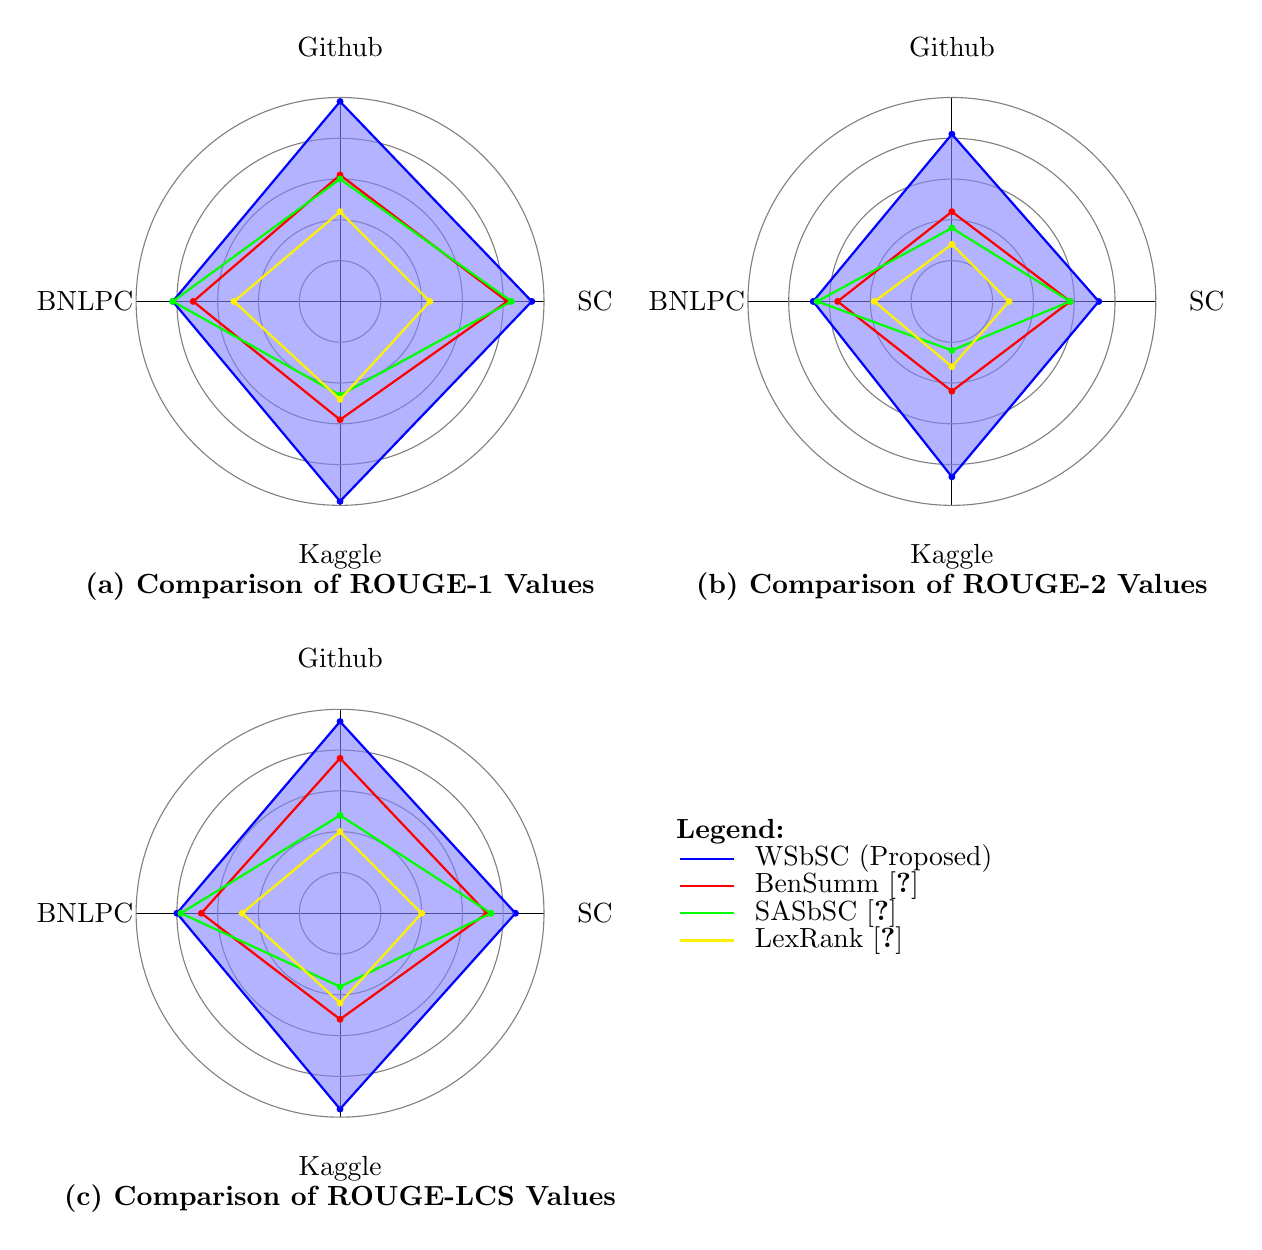
\begin{tikzpicture}[scale=0.0025*\textwidth]
    % Define the number of axes (dimensions)
    \def\n{4}
    % Define the names of the features
    \def\features{{"SC", "Kaggle", "BNLPC", "Github"}}
    % Define the maximum value
    \def\maxvalue{5}

    % Define values for three different radar charts
    \def\valuesAW{{4.7, 4.9, 4.1, 4.9}}
    \def\valuesAB{{4.1, 2.9, 3.6, 3.1}}
    \def\valuesAS{{4.2, 2.3, 4.1, 3.0}}
    \def\valuesAL{{2.2, 2.4, 2.6, 2.2}}

    \def\valuesBW{{3.6, 4.3, 3.4, 4.1}}
    \def\valuesBB{{2.9, 2.2, 2.8, 2.2}}
    \def\valuesBS{{2.9, 1.2, 3.3, 1.8}}
    \def\valuesBL{{1.4, 1.6, 1.9, 1.4}}

    \def\valuesCW{{4.3, 4.8, 4.0, 4.7}}
    \def\valuesCB{{3.6, 2.6, 3.4, 3.8}}
    \def\valuesCS{{3.7, 1.8, 3.9, 2.4}}
    \def\valuesCL{{2.0, 2.2, 2.4, 2.0}}

    % First Radar Chart (Top-left quarter)
    \begin{scope}[xshift=-5cm, yshift=5cm, scale=0.6]
        %write the dataset labels
        \foreach \i in {1,...,\n} {
            \draw (90-\i*360/\n:5) -- (0,0);
            \node at (90-\i*360/\n:6.25) {\pgfmathparse{\features[\i-1]}\pgfmathresult};
        }
        %draw the circle
        \node at (90-2*360/4:7){\textbf{(a) Comparison of ROUGE-1 Values}};
        \foreach \j in {1,...,\maxvalue} {
            \draw[gray, thin] (0,0) circle (\j);
        }

        %draw wsbsc
        \foreach \i [evaluate={\angle=90-\i*360/\n; \valueAW=\valuesAW[\i-1];}] in {1,...,\n} {
            \coordinate (PA\i) at (\angle:\valueAW);
            \filldraw[blue] (PA\i) circle (2pt);
        }
        \fill[blue!50, opacity=0.6] (PA1) -- (PA2) -- (PA3) -- (PA4) -- cycle;
        \foreach \i in {1,...,\n} {
            \pgfmathtruncatemacro{\nexti}{mod(\i,\n)+1}
%                    \draw [thick, cyan] plot [smooth, tension=2] coordinates { (PA\i) (PA\nexti)};
            \draw[thick, blue] (PA\i) -- (PA\nexti);
        }
%                \draw [thick,cyan] plot [smooth cycle, tension=1] coordinates { (PA1) (PA2) (PA3) (PA4)};

        %draw bensumm
        \foreach \i [evaluate={\angle=90-\i*360/\n; \valueAB=\valuesAB[\i-1];}] in {1,...,\n} {
            \coordinate (PB\i) at (\angle:\valueAB);
            \filldraw[red] (PB\i) circle (2pt);
        }
        \foreach \i in {1,...,\n} {
            \pgfmathtruncatemacro{\nexti}{mod(\i,\n)+1}
            \draw[thick, red] (PB\i) -- (PB\nexti);
        }

%                draw sasbsc
        \foreach \i [evaluate={\angle=90-\i*360/\n; \valueAS=\valuesAS[\i-1];}] in {1,...,\n} {
            \coordinate (PC\i) at (\angle:\valueAS);
            \filldraw[green] (PC\i) circle (2pt);
        }
        \foreach \i in {1,...,\n} {
            \pgfmathtruncatemacro{\nexti}{mod(\i,\n)+1}
            \draw[thick, green] (PC\i) -- (PC\nexti);
        }

        %draw lexrank
        \foreach \i [evaluate={\angle=90-\i*360/\n; \valueAL=\valuesAL[\i-1];}] in {1,...,\n} {
            \coordinate (PD\i) at (\angle:\valueAL);
            \filldraw[yellow] (PD\i) circle (2pt);
        }
        \foreach \i in {1,...,\n} {
            \pgfmathtruncatemacro{\nexti}{mod(\i,\n)+1}
            \draw[thick, yellow] (PD\i) -- (PD\nexti);
        }
    \end{scope}

    % Second Radar Chart (Top-right quarter)
    \begin{scope}[xshift=4cm, yshift=5cm, scale=0.6]
        \foreach \i in {1,...,\n} {
            \draw (90-\i*360/\n:5) -- (0,0);
            \node at (90-\i*360/\n:6.25) {\pgfmathparse{\features[\i-1]}\pgfmathresult};
        }
        \node at (90-2*360/4:7){\textbf{(b) Comparison of ROUGE-2 Values}};
        \foreach \j in {1,...,\maxvalue} {
            \draw[gray, thin] (0,0) circle (\j);
        }

        \foreach \i [evaluate={\angle=90-\i*360/\n; \valueBW=\valuesBW[\i-1];}] in {1,...,\n} {
            \coordinate (PA\i) at (\angle:\valueBW);
            \filldraw[blue] (PA\i) circle (2pt);
        }
        \fill[blue!50, opacity=0.6] (PA1) -- (PA2) -- (PA3) -- (PA4) -- cycle;
        \foreach \i in {1,...,\n} {
            \pgfmathtruncatemacro{\nexti}{mod(\i,\n)+1}
            \draw[thick, blue] (PA\i) -- (PA\nexti);
        }

        \foreach \i [evaluate={\angle=90-\i*360/\n; \valueBB=\valuesBB[\i-1];}] in {1,...,\n} {
            \coordinate (PB\i) at (\angle:\valueBB);
            \filldraw[red] (PB\i) circle (2pt);
        }
        \foreach \i in {1,...,\n} {
            \pgfmathtruncatemacro{\nexti}{mod(\i,\n)+1}
            \draw[thick, red] (PB\i) -- (PB\nexti);
        }

        \foreach \i [evaluate={\angle=90-\i*360/\n; \valueBS=\valuesBS[\i-1];}] in {1,...,\n} {
            \coordinate (PC\i) at (\angle:\valueBS);
            \filldraw[green] (PC\i) circle (2pt);
        }
        \foreach \i in {1,...,\n} {
            \pgfmathtruncatemacro{\nexti}{mod(\i,\n)+1}
            \draw[thick, green] (PC\i) -- (PC\nexti);
        }

        \foreach \i [evaluate={\angle=90-\i*360/\n; \valueBL=\valuesBL[\i-1];}] in {1,...,\n} {
            \coordinate (PD\i) at (\angle:\valueBL);
            \filldraw[yellow] (PD\i) circle (2pt);
        }
        \foreach \i in {1,...,\n} {
            \pgfmathtruncatemacro{\nexti}{mod(\i,\n)+1}
            \draw[thick, yellow] (PD\i) -- (PD\nexti);
        }
    \end{scope}

    % Third Radar Chart (Bottom-left quarter)
    \begin{scope}[xshift=-5cm, yshift=-4cm, scale=0.6]
        \foreach \i in {1,...,\n} {
            \draw (90-\i*360/\n:5) -- (0,0);
            \node at (90-\i*360/\n:6.25) {\pgfmathparse{\features[\i-1]}\pgfmathresult};
        }
        \node at (90-2*360/4:7){\textbf{(c) Comparison of ROUGE-LCS Values}};
        \foreach \j in {1,...,\maxvalue} {
            \draw[gray, thin] (0,0) circle (\j);
        }

        \foreach \i [evaluate={\angle=90-\i*360/\n; \valueCW=\valuesCW[\i-1];}] in {1,...,\n} {
            \coordinate (PA\i) at (\angle:\valueCW);
            \filldraw[blue] (PA\i) circle (2pt);
        }
        \fill[blue!50, opacity=0.6] (PA1) -- (PA2) -- (PA3) -- (PA4) -- cycle;
        \foreach \i in {1,...,\n} {
            \pgfmathtruncatemacro{\nexti}{mod(\i,\n)+1}
            \draw[thick, blue] (PA\i) -- (PA\nexti);
        }

        \foreach \i [evaluate={\angle=90-\i*360/\n; \valueCB=\valuesCB[\i-1];}] in {1,...,\n} {
            \coordinate (PB\i) at (\angle:\valueCB);
            \filldraw[red] (PB\i) circle (2pt);
        }
        \foreach \i in {1,...,\n} {
            \pgfmathtruncatemacro{\nexti}{mod(\i,\n)+1}
            \draw[thick, red] (PB\i) -- (PB\nexti);
        }

        \foreach \i [evaluate={\angle=90-\i*360/\n; \valueCS=\valuesCS[\i-1];}] in {1,...,\n} {
            \coordinate (PC\i) at (\angle:\valueCS);
            \filldraw[green] (PC\i) circle (2pt);
        }
        \foreach \i in {1,...,\n} {
            \pgfmathtruncatemacro{\nexti}{mod(\i,\n)+1}
            \draw[thick, green] (PC\i) -- (PC\nexti);
        }

        \foreach \i [evaluate={\angle=90-\i*360/\n; \valueCL=\valuesCL[\i-1];}] in {1,...,\n} {
            \coordinate (PD\i) at (\angle:\valueCL);
            \filldraw[yellow] (PD\i) circle (2pt);
        }
        \foreach \i in {1,...,\n} {
            \pgfmathtruncatemacro{\nexti}{mod(\i,\n)+1}
            \draw[thick, yellow] (PD\i) -- (PD\nexti);
        }
    \end{scope}

    % Legend (Bottom-right quarter)
    \begin{scope}[xshift=4cm, yshift=-4cm, scale=0.8]
        \node[anchor=west] at (-5.25, 1.5) {\textbf{Legend:}};
        \draw[thick, blue] (-5, 1) -- (-4, 1);
        \node[anchor=west] at (-3.8, 1) {WSbSC (Proposed)};

        \draw[thick, red] (-5, 0.5) -- (-4, 0.5);
        \node[anchor=west] at (-3.8, 0.5) {BenSumm~\cite{chowdhury-etal-2021-tfidf-clustering}};

        \draw[thick, green] (-5, 0) -- (-4, 0);
        \node[anchor=west] at (-3.8, 0) {SASbSC~\cite{roychowdhury-etal-2022-spectral-base}};

        \draw[thick, yellow] (-5, -0.5) -- (-4, -0.5);
        \node[anchor=west] at (-3.8, -0.5) {LexRank~\cite{Erkan-lexRank-2004}};
    \end{scope}
\end{tikzpicture}
    \caption{The Radar chart of the models of being compared on four datasets at once}
    \label{fig:radarchart}
\end{figure}
\begin{figure}
    \centering
    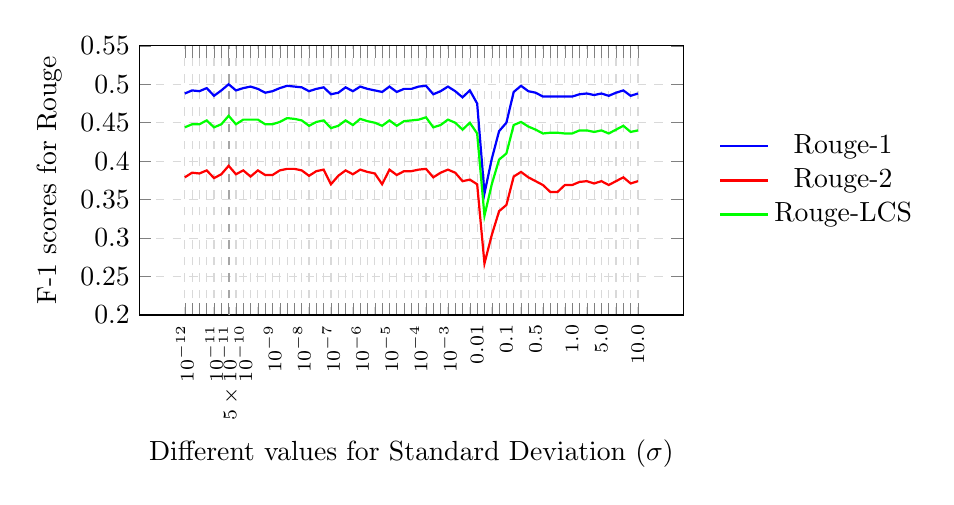
\begin{tikzpicture}
    \begin{axis}[
        width=.7\textwidth,
        height=5cm,
        xlabel={Different values for Standard Deviation ($\sigma$)},
        ylabel={F-1 scores for Rouge},
        ymin=0.2, ymax=0.55,
        xtick={1,2,...,63}, % Original 63 ticks
        xticklabels={ $10^{-12}$, , , , $10^{-11}$, ,$5\times10^{-11}$, , $10^{-10}$, , , , $10^{-9}$, , , , $10^{-8}$, , , ,
                     $10^{-7}$, , , , $10^{-6}$, , , , $10^{-5}$, , , , $10^{-4}$, , , ,
                     $10^{-3}$, , , , $0.01$, , , , $0.1$, , , , $0.5$, , , ,
                      , $1.0$, , , , $5.0$, , , , ,$10.0$}, % Show 1 in every 4 labels
        xticklabel style={rotate=90, anchor=east, font=\scriptsize}, % Rotate labels 90 degrees
        legend style={at={(1.05,0.5)}, anchor=west, draw=none}, % Move legend outside, remove border
        extra x ticks={7}, % Add extra tick for 7th position
        extra x tick style={grid=major, major grid style={gray!70, thick}}, % Style for the highlighted tic
        extra x tick labels={},
        grid=major,
        grid style={dashed,gray!30},
        ytick={0.20, 0.25, 0.30, 0.35, 0.40, 0.45, 0.50, 0.55}, % Y-axis ticks
        cycle list name=color list,
    ]

    % Dummy data for Column 1
    \addplot[color=blue, thick] coordinates {
        (1, 0.488)
        (2, 0.492)
        (3, 0.491)
        (4, 0.495)
        (5, 0.485)
        (6, 0.492)
        (7, 0.500)
        (8, 0.492)
        (9, 0.495)
        (10, 0.497)
        (11, 0.494)
        (12, 0.489)
        (13, 0.491)
        (14, 0.495)
        (15, 0.498)
        (16, 0.497)
        (17, 0.496)
        (18, 0.491)
        (19, 0.494)
        (20, 0.496)
        (21, 0.487)
        (22, 0.489)
        (23, 0.496)
        (24, 0.491)
        (25, 0.497)
        (26, 0.494)
        (27, 0.492)
        (28, 0.490)
        (29, 0.497)
        (30, 0.490)
        (31, 0.494)
        (32, 0.494)
        (33, 0.497)
        (34, 0.498)
        (35, 0.487)
        (36, 0.491)
        (37, 0.497)
        (38, 0.491)
        (39, 0.483)
        (40, 0.492)
        (41, 0.475)
        (42, 0.358)
        (43, 0.403)
        (44, 0.439)
        (45, 0.450)
        (46, 0.490)
        (47, 0.498)
        (48, 0.491)
        (49, 0.489)
        (50, 0.484)
        (51, 0.484)
        (52, 0.484)
        (53, 0.484)
        (54, 0.484)
        (55, 0.487)
        (56, 0.488)
        (57, 0.486)
        (58, 0.488)
        (59, 0.485)
        (60, 0.489)
        (61, 0.492)
        (62, 0.485)
        (63, 0.488)
    };
    \addlegendentry{Rouge-1}

    % Dummy data for Column 2
    \addplot[color=red, thick] coordinates {
        (1, 0.379)
        (2, 0.385)
        (3, 0.384)
        (4, 0.388)
        (5, 0.378)
        (6, 0.383)
        (7, 0.394)
        (8, 0.383)
        (9, 0.388)
        (10, 0.380)
        (11, 0.388)
        (12, 0.382)
        (13, 0.382)
        (14, 0.388)
        (15, 0.390)
        (16, 0.390)
        (17, 0.388)
        (18, 0.381)
        (19, 0.387)
        (20, 0.389)
        (21, 0.370)
        (22, 0.381)
        (23, 0.388)
        (24, 0.383)
        (25, 0.389)
        (26, 0.386)
        (27, 0.384)
        (28, 0.370)
        (29, 0.389)
        (30, 0.382)
        (31, 0.387)
        (32, 0.387)
        (33, 0.389)
        (34, 0.390)
        (35, 0.379)
        (36, 0.385)
        (37, 0.389)
        (38, 0.385)
        (39, 0.374)
        (40, 0.376)
        (41, 0.370)
        (42, 0.267)
        (43, 0.304)
        (44, 0.335)
        (45, 0.343)
        (46, 0.380)
        (47, 0.386)
        (48, 0.379)
        (49, 0.374)
        (50, 0.369)
        (51, 0.360)
        (52, 0.360)
        (53, 0.369)
        (54, 0.369)
        (55, 0.373)
        (56, 0.374)
        (57, 0.371)
        (58, 0.374)
        (59, 0.369)
        (60, 0.374)
        (61, 0.379)
        (62, 0.371)
        (63, 0.374)
    };
    \addlegendentry{Rouge-2}

    % Dummy data for Column 3
    \addplot[color=green, thick] coordinates {
        (1, 0.444)
        (2, 0.448)
        (3, 0.448)
        (4, 0.453)
        (5, 0.444)
        (6, 0.448)
        (7, 0.459)
        (8, 0.448)
        (9, 0.454)
        (10, 0.454)
        (11, 0.454)
        (12, 0.448)
        (13, 0.448)
        (14, 0.451)
        (15, 0.456)
        (16, 0.455)
        (17, 0.453)
        (18, 0.446)
        (19, 0.451)
        (20, 0.453)
        (21, 0.443)
        (22, 0.446)
        (23, 0.453)
        (24, 0.447)
        (25, 0.455)
        (26, 0.452)
        (27, 0.450)
        (28, 0.446)
        (29, 0.453)
        (30, 0.446)
        (31, 0.452)
        (32, 0.453)
        (33, 0.454)
        (34, 0.457)
        (35, 0.444)
        (36, 0.447)
        (37, 0.454)
        (38, 0.450)
        (39, 0.441)
        (40, 0.450)
        (41, 0.436)
        (42, 0.329)
        (43, 0.370)
        (44, 0.402)
        (45, 0.410)
        (46, 0.447)
        (47, 0.451)
        (48, 0.445)
        (49, 0.441)
        (50, 0.436)
        (51, 0.437)
        (52, 0.437)
        (53, 0.436)
        (54, 0.436)
        (55, 0.440)
        (56, 0.440)
        (57, 0.438)
        (58, 0.440)
        (59, 0.436)
        (60, 0.441)
        (61, 0.446)
        (62, 0.438)
        (63, 0.440)
    };
    \addlegendentry{Rouge-LCS}

    \end{axis}
\end{tikzpicture}
    \caption{Fine-tuning for different standard deviation~($\sigma$)~values}
    \label{fig:sigma-fine-tuning}
\end{figure}

\subsubsection{Different Sentence Extraction Techniques Inside Clusters} \label{subsubsec:different-ranking-techniques-inside-clusters}
We implemented two sentence extraction methods to pick the most representative sentence from each cluster. Firstly, the lead extraction method is used where we just select the sentence that appears first in the input document because generally the earlier sentences in an input has more information on the context of the input document. The second extraction method is the TF-IDF ranking method, where we ranked the sentences by their TF-IDF scores and picked the sentence with the most TF-IDF score. We can see in the table~\ref{tab:ranking} that the TF-IDF performs better on a high quality dataset like the self-curated dataset.

\begin{table}[]
    \centering
    \begin{tabular}{lccc}\hline
        Method      	& Rouge-1       & Rouge-2       & Rouge-LCS     \\\hline
        Lead extraction	& 0.47          & 0.36          & 0.43          \\
        TF-IDF ranking	& \textbf{0.50} & \textbf{0.40} & \textbf{0.46} \\\hline
    \end{tabular}
    \caption{Comparison of Result of different ranking techniques}
    \label{tab:ranking}
\end{table}

\subsection{Implementation Into Other Languages}\label{subsec:implementation-into-other-languages}
The proposed model is not language-dependent because it does not rely on any language specific features to summarize the input documents, thus it can be extended into other languages too. To implement this method into a language, we only need a language-specific tokenizer, a list of stop-words and a word vector embedding dataset. We implemented this model on three more languages to show the language independent nature of the model. To evaluate the quality of the sentence extraction, we tried to find evaluation datasets for summarization on other low resource languages, but could only find relevant datasets in three other languages. These languages are Hindi, Marathi and Turkish. We adopted the proposed model into these three low resource languages to check how well it performs.\\

\begin{table}[]
    \centering
    \begin{tabular}{lccc}\hline
        Language              	& Rouge-1   & Rouge-2   & Rouge-LCS \\\hline
        Bengali (Self-curated)	& 0.47      & 0.36      & 0.43      \\
        Bengali (Kaggle)   		& 0.49      & 0.43      & 0.48      \\
        Bengali (BNLPC)   		& 0.41      & 0.34      & 0.40      \\
        Bengali (Github)   		& 0.49      & 0.41      & 0.47      \\
        Bengali (Average)       & 0.47      & 0.38      & 0.44      \\\hline
        Hindi                   & 0.40      & 0.26      & 0.36      \\\hline
        Marathi                 & 0.50	    & 0.42      & 0.50      \\\hline
        Turkish                 & 0.48      & 0.39      & 0.47      \\\hline
    \end{tabular}
    \caption{Comparison of Result of proposed summarization method in other low-resource languages}
    \label{tab:other_language}
\end{table}

The Table-\ref{tab:other_language} shows the result of the proposed WSbSC method for extractive summarization in other low resource languages. In this table, We can see that the results on Marathi and Turkish are slightly better than the result on Bengali. Although it performs slightly lower on Hindi, The score is still similar to Bengali. To evaluate the result on Hindi language, we used a Kaggle dataset\footnote{\textit{https://www.kaggle.com/datasets/disisbig/hindi-text-short-and-large-summarization-corpus/}} produced by Gaurav Arora. For the Marathi language, we used another Kaggle dataset\footnote{\textit{https://www.kaggle.com/datasets/ketki19/marathi}} produced by Ketki Nirantar. For the Turkish language, we used a GitHub dataset\footnote{\textit{https://github.com/xtinge/turkish-extractive-summarization-dataset/blob/main/dataset/XTINGE-SUM\_TR\_EXT/xtinge-sum\_tr\_ext.json}} produced by the XTINGE~\cite{Demir-2024-xtinge_turkish_extractive} team for evaluation. 
